\section{系统分析}

\subsection{可行性分析}

本系统使用Django后端开发框架进行开发,开发环境在Ubuntu20.04操作系统下进行开发,基于Facenet的网络模型在Kaggle社区中提供的云计算平台进行训练,Kaggle社区为每个用户每周免费提供36个小时的加速计算平台,GPU硬件型号为Tesla P100,训练神经网络模型的框架使用PyTorch,以上所涉及到的编程框架以及开发环境都是开源的,所以在开发阶段并不需要投入过多的经济费用开支,而在开发完成之后的部署阶段,该系统即可选择云服务商提供的云主机进行部署,也可选择使用部署在其它服务器之上的系统。即使使用云服务商提供的云主机的方式进行部署,维护与租用费用都是完全可以接受的。从市场需求的角度来讲,现阶段大部分的中小型工厂企业所使用的的信息管理方式大多都为半手工半计算存储的方式来进行管理,使用本系统既可以解决手工管理信息的任务量大,也可以高效地对信息进行统一组织,并且将数据存储到云主机上,也可以有效防止信息丢失的问题。

\subsection{需求分析}

\subsubsection{业务需求分析}

1. 用户登录注册:在用户访问首页时,首先在访问请求中查询用户是否已经登录账号,之后根据登录与否,在页面顶部导航栏中显示欢迎用语或者显示登录按钮供用户登录。在注册页面,在用户填写注册信息之后,首先在用户终端使用JavaScript检测当前输入的信息格式是否正确,通过验证后发送请求到服务后端,再根据填写的信息进行进一步验证,例如验证电子邮件是否已经存在或组织名称是否冲突等,之后在数据库的用户表插入记录,存储用户信息,当注册成功之后,自动跳转到登录页面,之后登录流程如图\ref{fig:login}所示。

\begin{figure}[H]
    \centering
    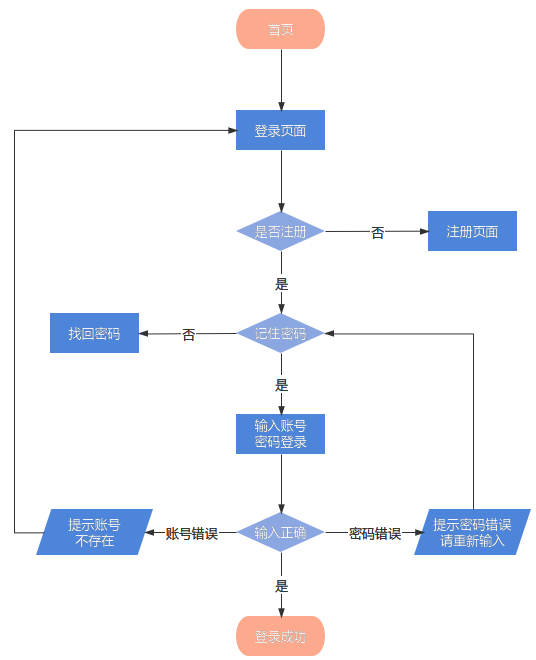
\includegraphics[width=.4\textwidth]{figures/3loginprocess.png}
    \caption{用户登录流程图}
    \label{fig:login}
\end{figure}

2. 信息管理:信息管理包括人员信息、产品信息和原材料信息。而人员信息管理又包括客户信息、员工信息以及供应商信息。管理人员对工厂信息进行管理时,首先进入到管理页面,然后根据信息管理页面,输入新建的实体信息,之后后端系统查询数据库是否存在信息冲突或不一致等问题,向管理人员输出管理信息提示,成功新建之后,向数据库添加记录,如图\ref{fig:3ifmtmngmt}所示。

\begin{figure}[H]
    \centering
    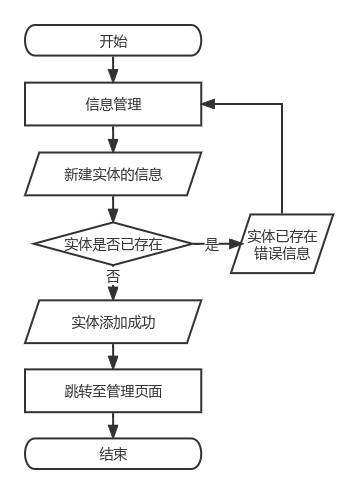
\includegraphics[width=.35\textwidth]{figures/3ifmtmngmt.png}
    \caption{工厂信息管理流程图}
    \label{fig:3ifmtmngmt}
\end{figure}

3. 客户下单:当客户对工厂所生产的产品有供货需求时,可以进入客户信息管理页面,对指定客户进行下单操作,之后在下单页面中,输入指定的产品以及产品数量进行下单,如图\ref{fig:3odmngmt}所示。

\begin{figure}[H]
    \centering
    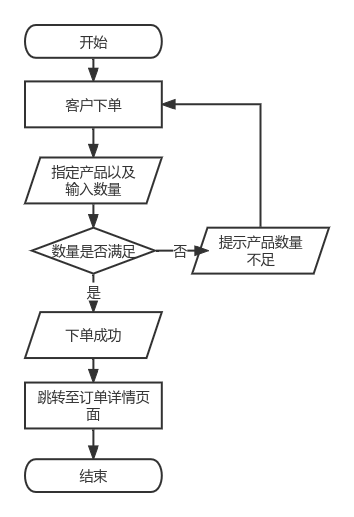
\includegraphics[width=.35\textwidth]{figures/3odmngmt.png}
    \caption{客户下单流程图}
    \label{fig:3odmngmt}
\end{figure}

4. 购买原材料:在生产环境中,当某一种原材料余量不足时,管理人员需及时购入原材料。在购买原材料页面,管理人员需要选择供应商、原材料类型和数量,之后检查当前工厂余额是否满足,之后完成对原材料的购买操作,如图\ref{fig:3brmtra}所示。

\begin{figure}[H]
    \centering
    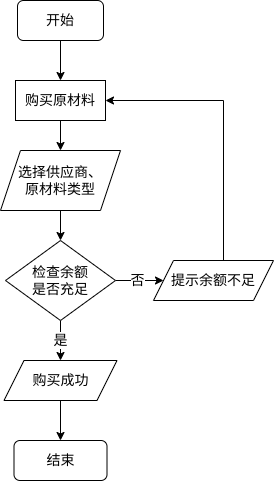
\includegraphics[width=.35\textwidth]{figures/3brmtra.png}
    \caption{购买原材料流程图}
    \label{fig:3brmtra}
\end{figure}

5. 员工签到:在工厂后勤管理中,对员工进行考核签到,该系统可使用人脸识别对员工身份进行认证,若认证失败,提示员工调整人脸角度等重新识别;若成功认证,将签到记录插入到签到表中完成员工签到功能,如图\ref{fig:3fcrcgnt}所示。

\begin{figure}[H]
    \centering
    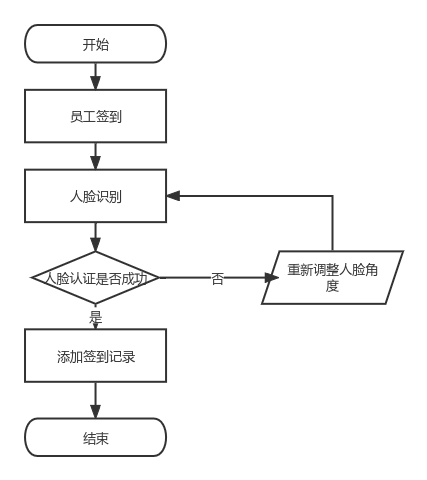
\includegraphics[width=.45\textwidth]{figures/3fcrcgnt.png}
    \caption{员工签到流程图}
    \label{fig:3fcrcgnt}
\end{figure}

\subsubsection{功能性需求分析}

1. 工厂管理员:管理员对工厂信息进行管理时,包括交易记录、员工信息、客户信息、供应商信息、产品信息和原材料信息等。在对原材料信息进行管理时,还需要添加根据供应商来购入指定的原材料,由管理人员录入需要购入的价格以及重量等信息。在对员工进行考勤时,使用人脸识别对员工识别并且进行签到,将信息存储到签到表。系统的用例图如图\ref{fig:usecase}所示。

\begin{figure}[H]
    \centering
    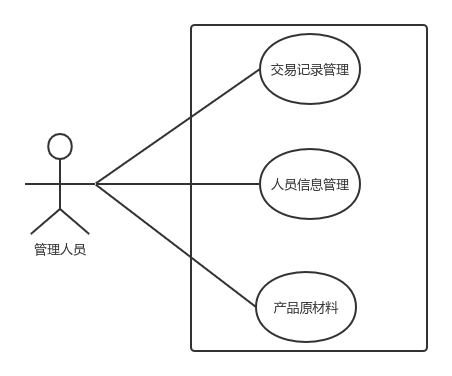
\includegraphics[width=.55\textwidth]{figures/3usecase.png}
    \caption{工厂管理员用例图}
    \label{fig:usecase}
\end{figure}

2. 客户:在涉及到客户信息管理,除了客户个人信息之外,还需要包括对指定客户根据产品以及重量信息的下单功能进行设计。还需根据客户的订单状态,分别查看已送达的订单和未送达的订单,对订单进行管理,如图\ref{fig:3cstmusecase}所示。

\begin{figure}[H]
    \centering
    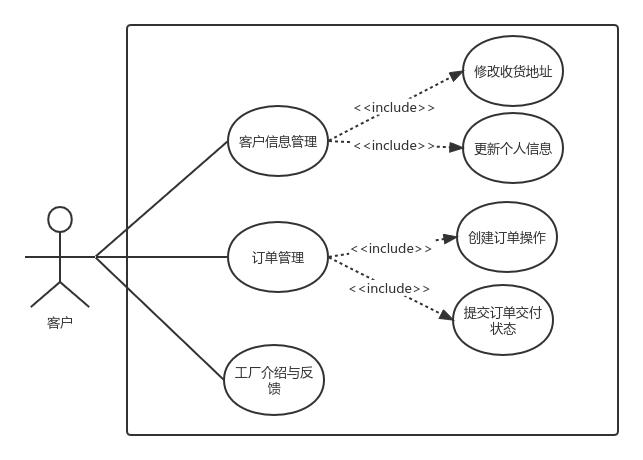
\includegraphics[width=.75\textwidth]{figures/3cstmusecase.png}
    \caption{客户用例图}
    \label{fig:3cstmusecase}
\end{figure}

3. 员工:对员工信息进行管理时,除了员工的个人信息以外,还需要对指定员工进行下达工作任务,例如指定制作的产品、使用的原材料和生产重量等;还包括对员工的薪资进行支付等操作,如图\ref{fig:3empleusecase}所示。

\begin{figure}[H]
    \centering
    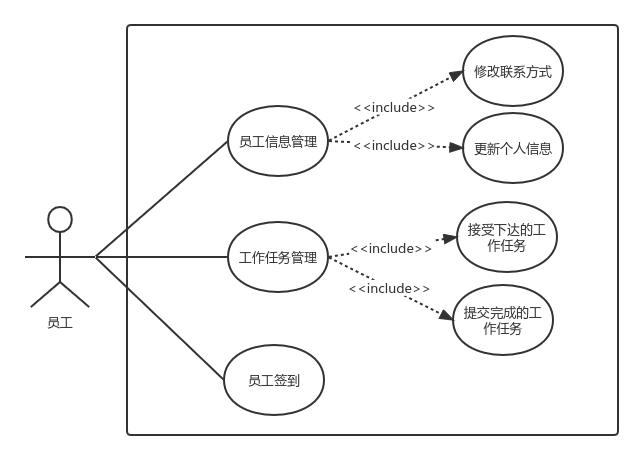
\includegraphics[width=.75\textwidth]{figures/3empleusecase.png}
    \caption{员工用例图}
    \label{fig:3empleusecase}
\end{figure}

\subsubsection{非功能性需求分析}

1. 系统环境:Ubuntu 20.04

2. 开发语言发行版本:Miniconda 3、Python 3.6。

3.依赖环境版本:Django 3.2.13、facenet-pytorch 2.5.2、numpy 1.21.5、Pillow 9.1.0、tensorboard 2.8.0、torch 1.11.0、torchvision 0.12.0。

4. 系统可扩展性:系统在投入正式运行后,若用户有新的需求,系统需要增加新的功能模块并更新系统,以此保证系统能够顺利运行和发展。


% \subsubsection{人脸识别签到}

% 管理员对员工进行考核时,使用人脸识别对输入图像进行扫描,将根据人脸识别模块的输出对应的员工信息进行签到记录,将记录插入到员工签到表。对于人脸识别系统\cite{deepfrsurvey},有3个不可或缺的组成部分如图\ref{fig:facerec}所示。

% \begin{figure}[H]
%     \centering
%     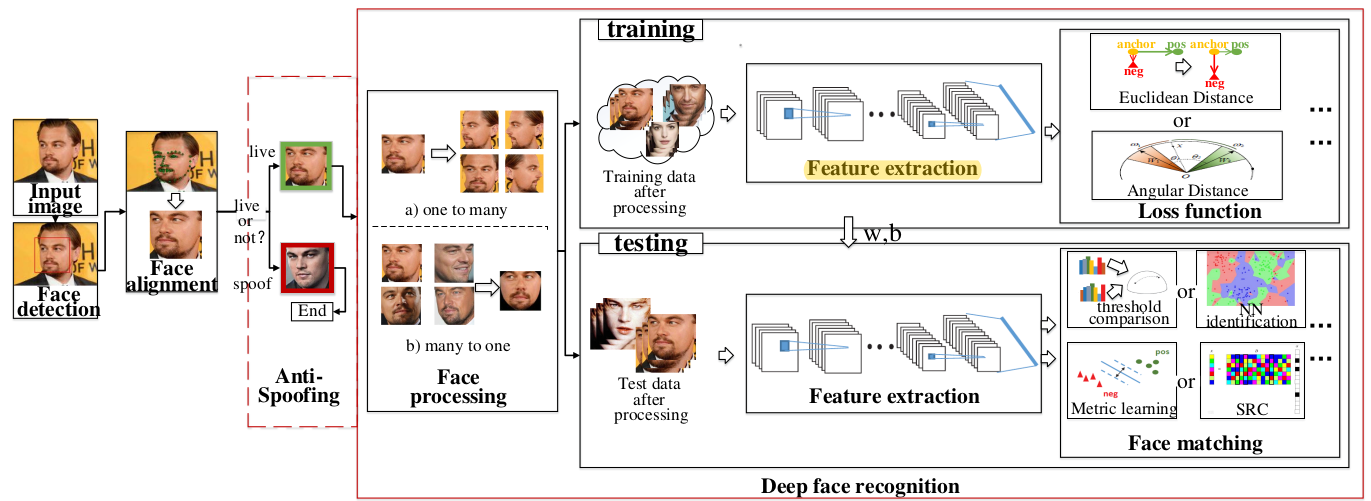
\includegraphics[width=\textwidth]{figures/3facerec.png}
%     \caption{人脸识别系统组成部分}
%     \label{fig:facerec}
% \end{figure}

% 首先,使用人脸检测模块对输入的图像或视频进行人脸检测,返回当前输入的图像或视频是否存在人脸。之后使用人脸对齐模块,对输入图像中的人脸进行关键点检测,将图像中的人脸部分对齐规范到标准坐标中。将人脸对齐模块的输出图像输入到特征提取模块,通常为深度卷积神经网络进行特征提取。将提取出的特征输入到最后的人脸匹配模块,用于将当前输入的图像与人脸数据库中的图像特征进行匹配比较,通常有阈值比较、K近邻识别、指标学习和SRC等。